\newpage
\subsection{Basic Fish}
\label{X-Wing}
Die Techniken \textit{X-Wing}, \textit{Swordfish} und \textit{Jellyfish} sind die einfachsten Unterarten der Fische. Sie funktionieren nach dem selben Prinzip, nur dass eine unterschiedliche Anzahl an Figuren betrachtet wird, ähnlich zu \textit{Naked Subset} und \textit{Hidden Subset}. Hier wird stellvertretend die Technik \textit{X-Wing} erklärt und am Beispiel gezeigt.\\
Dazu sucht man zwei Spalten oder Zeilen, die ausschließlich in den selben zwei Zellen einen bestimmten Kandidaten, die Fischziffer, beinhalten. Nun kann man aus dem jeweils anderen Paar von Figuren (Spalte oder Zeile), deren Position durch die zwei gefundenen Zellen festgelegt wird, alle Fischziffern löschen, die nicht gleichzeitig in einer der zuerst ausgesuchten Figuren liegen.\\
Da die Fischziffer in den beiden zuert ausgesuchten Figuren nur an jeweils zwei Stellen liegen kann und diese sich paarweise gegeinseitig ausschließen ist klar, dass jedes Vorkommen der Fischziffer in den zuletzt ausgesuchten Figuren in der Überschneidung mit den ersten Figuren liegen muss.

\begin{figure}[h]
\begin{center}
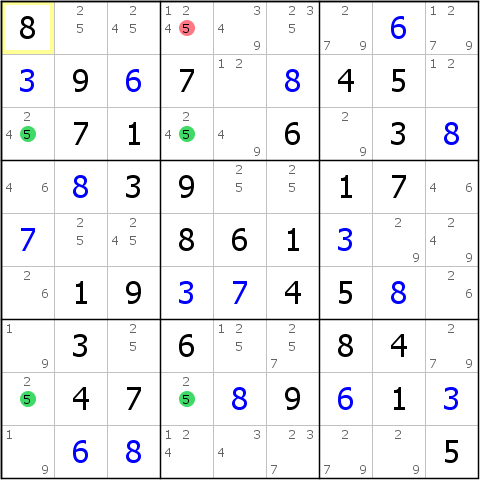
\includegraphics{./img/x_wing.png}
\caption{Basic Fish - X-Wing}
\end{center}
\end{figure}

Ein Beispiel für die Technik \textit{X-Wing} findet sich in \textbf{Abbildung 3.8}. Hier wurden als erste Figuren die Zeilen 2 und 5 gewählt. Diese enthalten die Fischziffer 5 nur an den Stellen 5 und 8. Wichtig ist, dass es in den beiden Zeilen die gleichen Positionen sind. Da die Ziffer 5 und Zeile 2 nur an den Positionen 5 und 8 stehen kann werden beiden Fälle nun gtrennt betrachtet. Steht in z2s5 die Ziffer 5, dann muss sie auch in z5s8 stehen, da sonst die Zeile 5 die Ziffer 5 nicht enthalten würde. Umgekehrt gilt:Steht in z2s8 die Ziffer 5, dann muss sie auch in z5s5 stehen. In jedem der beiden möglichen Fälle gilt, dass sowohl in Spalte 5 als auch in Spalte 8 die Ziffer 5 vorkommt und zwar in den Zeilen 2 und 5. Daher kann aus allen anderen Zellen der Spalten die Fishziffer 5 gelöcht werden, falls sie in den Kandidatenlisten vorhanden ist.